\chapter{Securing the OBD-II port}
\label{chap:solution}

In this chapter, a proposal is presented that attempts to address the security issues of OBD-II. This system employs the security solutions presented in Chapter \ref{chap:preliminaries}. More specifically, the concept of RBAC is applied to the OBD-II interface by introducing public key cryptography. First, a suitable attacker model is defined. Second, a general description of the ideal OBD-II system is presented (i.e. a OBD-II system that doesn't suffer from all the problems mentioned in Section \ref{sec:motivation}). In the last part of this chapter the design of the proposed solution is discussed.

\section{Attacker model} 
\label{sec:attacker_model}

To further characterize the security issues of OBD-II, it is useful to specify an attacker model. This model serves as a survey of the attacker's capabilities and motives; thus, defining a set of criteria on which potential countermeasures can be judged. A typical attacker will not necessarily conform to all these characteristics, but the idea is that any countermeasure would have to address them nonetheless. First, the different types of attacks that are possible are discussed. Second we will look at which type of individuals could perform these attacks, and what motivates them to do so. In the last part of the attacker model, we provide a series of examples illustrating a typical OBD-II attack via physical access.

\subsection{Type of Attack}  
\label{subsec:attack_type}

All of the example attacks presented later in Section \ref{subsec:example_attacks} were leveraged by gaining physical access to the vehicle. This situation is illustrated in Figure \ref{fig:attackmodel_1}. Physical access is ideally only granted to the owner of the vehicle, and it's safe to assume that (s)he is not intent on mounting an attack on their own vehicle. However, It is not unthinkable for an attacker to gain access illegally (e.g. car theft) or by abusing privileges that were bestowed on them by the owner (e.g. a repairman). While physical access is the most evident way of mounting an attack via the OBD-II interface, another alternative is certainly worth examining. In this approach an attacker would abuse the connection of an extant OBD-II communication by hijacking the session. When the session is physical in nature (i.e. a user directly interfacing with the OBD-II system via a hand-held device) this scenario is unlikely, since the user would be aware of any malicious third parties. When we consider that the session can be wireless however, like the DLC connector with wifi/Bluetooth capabilities discussed in Section \ref{subsec:obd:pid}, this scenario becomes increasingly likely. Especially since the wireless capabilities of diagnostics systems will only increase in the future, as is discussed in \cite{Kleberger}. This situation is illustrated in Figure \ref{fig:attackmodel_2}.


\begin{figure}[h]
	\centering
	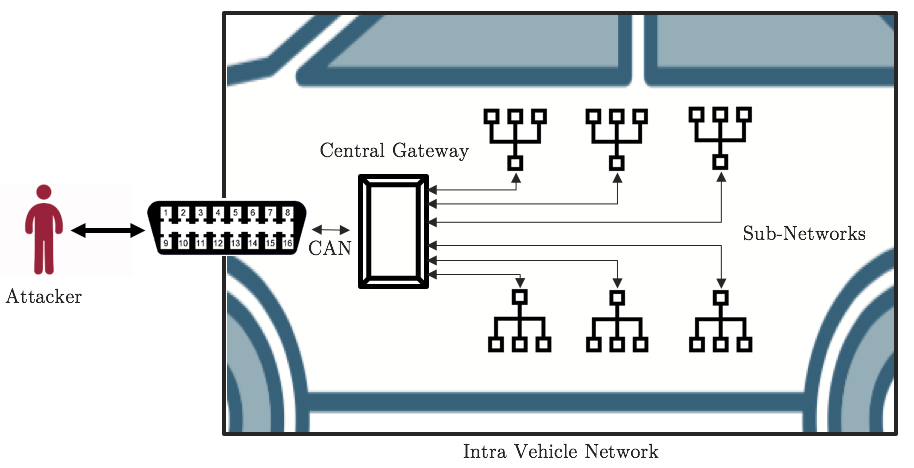
\includegraphics[width=\textwidth]{attackmodel_1.png}
	\caption{Attacker with physical access.}
	\label{fig:attackmodel_1}
\end{figure}

\begin{figure}[h]
	\centering
	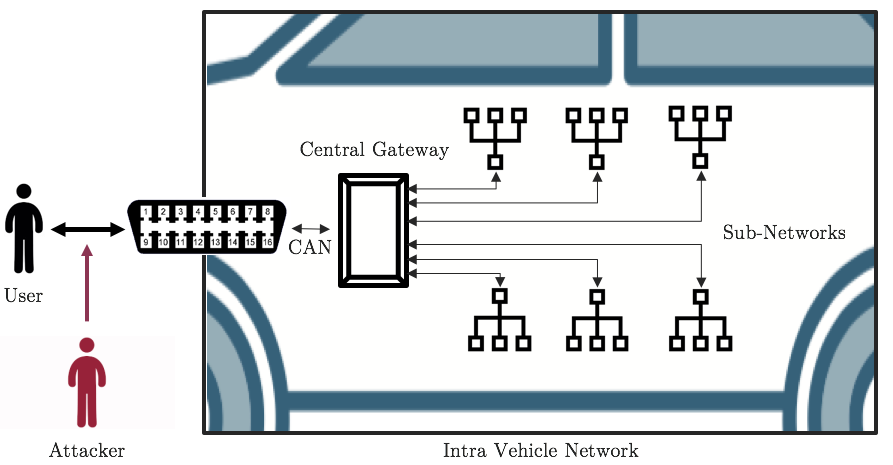
\includegraphics[width=\textwidth]{attackmodel_2.png}
	\caption{Attacker hijacking another OBD-II session.}
	\label{fig:attackmodel_2}
\end{figure}

\subsection{Type of Attacker}
\label{subsec:attacker_type}

Aside from the type of attacks that are possible, it is valuable to define which type of attackers would be interested in attempting them and why. The European Union Agency for Network and Information Security (ENISA) defines 4 types of cyberattacks on smart cars in \cite{Enisa}: 

\begin{itemize}
	\item \textbf{Attacks targeting driver/passenger safety:} This is probably the most serious and harmful type of attacks, since they directly involve the safety of the passengers. Why anyone would be motivated to jeopardize the well-being of another person can vary: extortion, financial gain, rivalries, etc. In the context of OBD-II it is the second attack scenario (i.e. remote OBD-II session hijacking) that is especially relevant here, since these would allow an adversary to initiate the attack while the vehicle is on the road. However, it is not entirely unlikely that someone would compromise the vehicle via the OBD-II interface beforehand, with the intention of compromising drivers/passenger in the future.
	
	\item \textbf{Persistent vehicle alteration by legitimate users:} Most car owners will never concern themselves with the OBD-II interface, and might not even know it exists. Others however, albeit out of sheer curiosity, might take an interest and discover all the possibilities that the OBD-II interface has to offer. These 'automotive network adventurers' could inadvertently compromise the integrity of the network, thereby endangering themselves and all their passengers. Another incentive for people to alter the behaviour of their own vehicle is personal gain: lowering the internal odometer value before selling the vehicle, clearing recent crash data to fool insurance companies, recalibrating sensors to pass emissions tests, improving the performance of the engine, etc.  
	
	\item \textbf{Surveillance:} The DLC connector with wifi/Bluetooth capabilities presented in Section \ref{subsec:obd:pid} enables adversaries to remotely monitor the position of the vehicle, and by extension the driver and passengers. This could be taken even further if the GPS system could be remotely compromised. There are many reasons why an adversary or an organisation would be interested in collecting vehicle locations; depending on the type of surveillance: 
	\begin{itemize}
		\item \textbf{Targeted surveillance:} Where tracking is facilitated by exploiting a vulnerability of a specific individual's vehicle. The effort and cost involved in such an operation hints at the following motives: espionage, crime, terrorism, or business intelligence.
		
		\item \textbf{Mass surveillance:} where a great number of individuals are tracked by exploiting some common vulnerability. Because of the scope these types of attacks, it is likely they are issued by government agencies and criminal organisations.
	\end{itemize}
	
	
	\item \textbf{Theft:} While exploiting remote keyless entry (RKE) vulnerabilities (see Section \ref{subsubsec:rke}) and replaying Radio Frequency identification (RFID) signals (see Section \ref{subsubsec:rfid}) are more common ways of stealing cars, it is not entirely unlikely for the OBD-II interface to be exploited as well. For example, a resourceful adversary could inject a series of messages via the OBD-II interface; tricking the vehicle into starting the ignition.	
\end{itemize}
To sum up, our solution should defend against two different attack scenarios: direct physical access and remote session hijacking. Additionally, we must not underestimate the resources and capabilities of potential attackers. Since, they could range from an inquisitive vehicle owner, to an entire company or government agency. Also, the impact of these attacks can vary from essentially harmless, to physically endangering drivers and their passengers; indicating that care must be taken to design a system that is sufficiently secure. To further illustrate the security vulnerabilities of OBD-II, a series of example attacks are presented in the next section.

\subsection{Example attacks}
\label{subsec:example_attacks}

The exploits that are presented here were performed by Charlie Miller and Chris Valasek and documented in \cite{MillerC}; in an effort to raise awareness about the issue, as well as allowing car manufacturers to build safer cars in the future. They accomplished this by not only finding and exploiting various vulnerabilities in extant vehicles, but also sharing any software that made these exploits possible. An example of this is EcomCat, which is software written to aid in the reading and writing of data to the CAN bus through one or more Ecom cables \cite{MillerC}. The Ecom cable is then used to connect a laptop to the OBD-II DLC; allowing the researchers to use their EcomCat software to inject their own CAN messages onto the internal bus. Although seemingly straightforward, there are many potential problems in attempting to make the vehicle perform actions by injecting packets on the CAN bus. First, not everything can be controlled via the CAN bus (e.g. cruise control). Second, if a specific type of CAN packet is found to be a request (An ECU asking for another ECU to perform an action), replaying a fake copy does not guarantee that the message is accepted. This is because the original message is still sent; possibly confusing the ECU with conflicting information. Third, It is also possible that fake messages are ignored because of built-in security features inside the ECU. Despite these difficulties, these researchers did manage to mount a series of interesting exploits, three of which are presented here next.

\subsubsection{Speedometer} 
\label{subsubsec:speedometer}

In this example, performed on a 2010 Toyota Prius, the researchers managed to identify the messages that are sent to the speedometer to display the current velocity of the vehicle. Replaying this message with custom data fields allowed them to display any arbitrary speed on the speedometer display.

\subsubsection{Denial of Service} 
\label{subsubsec:denial_of_service}

Here the researches cleverly take advantage of how the CAN protocol works. Remember from Section \ref{subsec:can:message_arbitration} that CAN uses priority scheduling over the ID's of the messages that are sent on the bus. This means that spamming a high priority message would prevent all other messages from being transmitted. This vulnerability is exploited here by flooding the bus with CAN messages with an ID of 0. This flooding of the CAN bus halts the engine from being turned on, as well as putting the system in an all out state of disarray.

\subsubsection{Diagnostic session} 
\label{subsubsec:diagnostic_session}

The aforementioned examples used injection of messages that are normally sent from ECU to ECU, thereby erroneously invoking certain actions. Another approach is to trick the vehicle network into starting a diagnostic session; these are used in normal circumstances by a technician at a garage. It allows them to test the function of an ECU without having to take the vehicle on the road, as well as recalibrating them. Starting a diagnostic session does require circumventing an authentication procedure (see Section \ref{sec:obd_access_control}); however, this proved rather easy (this was done by reverse engineering an official authentication device and extracting the keys). Once a diagnostic session was established, it opened up a wide array of possible attacks: killing the engine, disabling the brakes, honking the horn, unlocking/locking doors, and even reprogramming of certain ECU's (see \cite{MillerC} for a detailed description of the attacks).

\section{Ideal OBD-II System}
\label{sec:sol_RBAC}

The research question of this thesis paper is: can a solution be developed that would protect an in-vehicle network from unauthorised access via the OBD-II port? The concept of 'unauthorised access' is key, since the goal is not to deny access altogether. Only authorised personnel (e.g. repairmen) should be allowed high levels of access, since only they should be allowed to start diagnostic sessions, recalibrate ECU's, etc. The only way of differentiating between what is allowed and what is not, is by looking at the messages that are sent, specifically their ID's. Some messages, like a message asking for the status of a certain ECU, could be considered harmless. The message that is used to initiate a diagnostics session however is not that innocent, since it is shown in \cite{MillerC} that this could be used to disengage the brakes, kill the engine, etc. It follows that any solution to this problem should involve a series of authorisation levels, and that each one of these roles should associated with a number of permitted message ID's. The concept of role-based access control presented in Section \ref{sec:RBAC} is clearly applicable here. \\ \\ The next question to answer is: where should this system of access control be enforced? The assertion made in Section \ref{sec:motivation}, stating that the main problem of OBD-II is the indiscriminate nature at which the gateway forwards messages coming from the interface, hints at the ideal solution. Because of it's strategic position and privileged role in forwarding messages, the gateway is the ideal location to enforce a RBAC system for OBD-II. Another reason for this is the fact that our solution should be software based, as is discussed in Section \ref{sec:challenges}. A solution that requires the introduction of dedicated hardware, would result in a system that is difficult to implement in practice. Indeed, it would require significant cost and effort from car manufacturers to modify the hardware of millions of currently in-use vehicles. A software update of extant gateway ECU's on the other hand, requires significantly less effort. \\ \\ The final question is how to enforce RBAC in practice. In a common enterprise RBAC system, the worker authenticates to the system via some type of authentication key. this key can be literally: physical key, key-card, software key, etc. However, in some instances this key is represented by some type of secret knowledge (like a password or PIN-code) or even some identifying characteristic of the individual (fingerprint scan, retinal scan, etc). The  worker authenticates to the system by proving (s)he is in possession of the appropriate key. Translating this concept to our situation; the user (e.g. car owner, repairman, policeman, etc) authenticates to the system (the gateway of the vehicle) by proving that (s)he in possession of the appropriate key. The system will verify this key before granting the permissions that correspond to the appropriate role. It should come as no surprise that an authentication scheme based on software keys is appropriate here. \\ \\ Every authorisation level constitutes a role, and what messages are allowed for each level constitute the permissions of this role. More specifically, this system should be considered an instance of mandatory access control (see Section \ref{sec:RBAC}), since the users are not allowed any control over what permissions they are granted. Now that a system of access control is introduced, we need to look at how this system can be implemented to protect the OBD-II port.

\section{OBD-II Access Control}
\label{sec:obd2_access_control}

It is time to present our solution. Our proposal constitutes a RBAC system for the OBD-II interface, that employs asymmetric key pairs to authenticate users. This system is illustrated in Figure \ref{fig:solution}. The choice was made to make use of cryptographic keys to implement access control. This means that users will have to prove they are in possession of the appropriate cryptographic key, in order for them to gain access to the vehicle network. Introducing a single cryptographic key that grants access to all extant vehicles is considered infeasible (requiring all vehicle manufacturers to cooperate), as well as insecure (disclosure of this single key would result in the exposure of all vehicles). This is why we propose to introduce different cryptographic keys for every vehicle model. From Section \ref{sec:PKC} it follows that there are two distinct cryptographic key technologies that can be considered: symmetric and asymmetric. Symmetric cryptography has the advantage of shorter key lengths and faster calculations, however this would entail that if the keys of one vehicle were extracted and distributed (e.g. by physically analysing the gateway), all vehicles of the same model would be compromised. That is why the decision was made to use asymmetric keys for authentication, as well as generating a temporary symmetric key. This symmetric key can then be used to secure the following communications session against session hijacking. \\ \\ The gateway stores a series of public keys, each one associated with a specific role. A user wishing to authenticate him/herself would have to prove the ownership of the appropriate private key.\footnote{This key ownership configuration could be flipped (i.e. gateway stores private key and user owns public key). However, this configuration has the same major design flaw that symmetric encryption had, namely possible extraction of the private key from the vehicle} The decision to use asymmetric keys moves the responsibility of safely storing the private key to the users. Intuitively this might seem like a bad idea, since now the private keys are already in the hands of individuals; individuals that might have ulterior motives concerning their level of access. This flaw was countered by introducing a central server that safely stores the private keys, together with an internet connected device called a tester that physically connects to the OBD-II port. Users with privileged roles will first authenticate to the central server via the tester, using some other authentication method (e.g. login and password). This dedicated device will then initiate an authentication procedure with the gateway, proving ownership of the appropriate private key while also establishing a shared secret. This authenticated key agreement procedure is discussed in more detail next.

\begin{figure}[h]
	\centering
	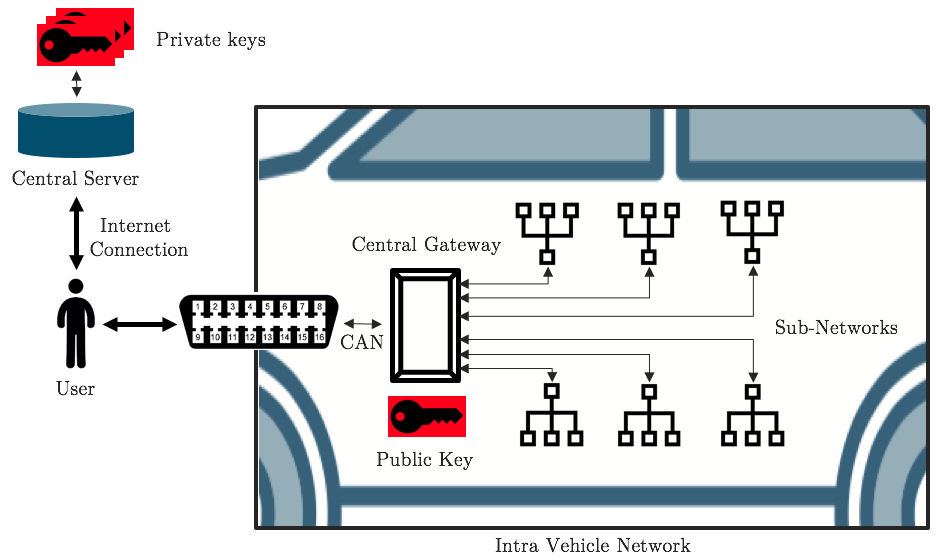
\includegraphics[width=\textwidth]{solution.png}
	\caption{OBD-II access control architecture.}
	\label{fig:solution}
\end{figure}


\subsection{Authenticated Key Agreement Procedure}
\label{subsec:authenticated_key_agreement_procedure}

The goal of the authenticated key agreement procedure is to prove to the gateway that the user is in possession of the appropriate private key, while also facilitating an authenticated session between tester and gateway by calculating a shared secret key. This calculation will incorporate the pre-shared asymmetric keys, thereby combining authentication and secret key establishment into a single procedure. This procedure is based on the ECDHE\_ECDSA algorithm introduced in Section \ref{subsubsec:ecdh_ecdsa}, specifically Figure \ref{fig:ECDH2}. A couple of changes were applied to this algorithm to more closely adhere to our situation:
\begin{enumerate}
	\item \textbf{Gateway Key Pair:} A precondition for the ECDHE\_ECDSA algorithm is that both parties have an ECC key pair already established. For the tester this condition is already met; even better, the corresponding public key is already given to the gateway. However, for the gateway this is not the case. ECDH requires two key pairs, so a new key pair will have to be computed every time the procedure is run.
	
	\item \textbf{Perfect Forward Secrecy:} We can get rid of the ephemeral keys. This is because perfect forward secrecy (or secrecy in general) is not a goal in our situation. the goal is to protect against unauthorised access, not to protect past sessions from leaking. 
	
	\item \textbf{Mutual Authentication:} The first authentication step can be omitted (i.e signing by the gateway, and verification by the tester). Because of the absence of a gateway key pair, it is impossible for the gateway to authenticate itself to the tester. Moreover, this is not even a requirement of our authentication procedure.
\end{enumerate}
Considering these modifications, the procedure from Figure \ref{fig:authentication_procedure} is obtained. Before the procedure is initiated, the central server is in possession of the OBD-II private key $Pr_{obd}$, while the gateway has the corresponding public key $Pb_{obd}$ stored in memory. The user of the tester initiates the procedure by connecting to the OBD-II port, after which the tester sends an initialization message to the gateway. This initialization message also specifies the role that the user of the tester wishes to authenticate as. The gateway responds to this by creating a new ECC key pair: KGen($Pb_g$,$Pr_g$), and sending the newly created public key $Pb_g$ to the tester. The tester then forwards this secret key to the central server, which in turn signs this public key using the OBD-II private key: Sig($Pb_g$,$Pr_{obd}$), before sending the signature back to the tester. The tester then forwards this signature (only the signature) back to the gateway. After the gateway has verified the signature using the OBD-II private key: Ver(Sig,$Pb_{obd}$), both parties calculate the shared secret using ECDH. The gateway does this by calculating $K$=ECDH($Pr_g$,$Pb_{obd}$). The tester however does not have all the ingredients to do so, since the OBD private key is stored on the central server. That is why the shared secret is generated on the server, before being securely transmitted to the tester. This newly created secret can then be used by both communicating parties to authenticate every OBD-II message that is sent in the upcoming session; this procedure is discussed next.
 
\begin{figure}[h]
	\centering
	\fbox{
		\procedure{OBD-II authenticated key agreement procedure}{%
			\textbf{Central Server} \<\< \textbf{Tester}  \<\< \textbf{Gateway} \\
			\text{$Pr_{obd}$} \<\<\<\< \text{$Pb_{obd}$} \\
			\<\< \< \sendmessageright{length=1.5cm,top=\text{init}} \<\\
			\<\<\<\< \text{KGen($Pb_g$,$Pr_g$)} \\
			\<\sendmessageleft{length=1.5cm,top=\text{$Pb_g$}} \<\< \sendmessageleft{length=1.5cm,top=\text{$Pb_g$}} \<\\
			\text{$S$=Sig($Pb_g$,$Pr_{obd}$)} \<\<\<\< \\
			\< \sendmessageright{length=1.5cm,top=\text{$S$}} \<\< \sendmessageright{length=1.5cm,top=\text{$S$}} \<\\
			\<\<\<\< \text{Ver($S$,$Pb_{obd}$)} \\
			\text{$K$=ECDH($Pr_{obd}$,$Pb_g$)} \< \sendmessageright{length=1.5cm,top=\text{$K$}} \<\<\< \text{$K$=ECDH($Pr_g$,$Pb_{obd}$)} \\
		}
	}
	\caption{OBD-II authenticated key agreement procedure}
	\label{fig:authentication_procedure}
\end{figure}

\subsection{Message Authentication Procedure}
\label{subsec:message_authentication_procedure}

The authentication procedure from Section \ref{subsec:authenticated_key_agreement_procedure} authenticates the tester to the gateway, thereby also establishing a shared secret. The next step is to design a procedure that uses this shared secret to facilitate an authenticated communications session. The solution proposed by the researchers of this paper is simple, and is illustrated in Figure \ref{fig:message_authentication}. The OBD-II message $M$ sent by the tester is followed up by a message containing a MAC: MAC($M$,$K$) (see Section \ref{subsec:MAC}). This MAC is calculated by inputting the data of the first CAN frame as well as the recently established secret key $K$. Before the gateway forwards the message to the appropriate sub-network, it first performs two distinct security checks: 
\begin{itemize}
	\item \textbf{Permissions Check} CheckP($M$): This is where the security policy of the role based access control system proposed in Section \ref{sec:sol_RBAC} is enforced. The user specified his/her role in the initialization message, so the gateway knows the role of the user. The first condition that is checked is whether this role has permission to send the message $M$. It will do this by looking up the ID of the message in the permission table (see Section \ref{subsec:permissions_table}). If the role does not have the permission to send the message, it will be denied and the tester (and by extension the user) is notified.
	
	\item \textbf{MAC Verification} Ver(MAC,$K$): After the message $M$ passes the permissions check, the gateway will check whether the received MAC is correct; ensuring that the sender of this message is authorized. Again, if this test fails the message will be denied and the tester is notified
\end{itemize}
If both these checks succeed, the OBD-II message $M$ is forwarded to the appropriate sub-network and the tester receives an acknowledgement (ACK). 

\begin{figure}[h]
	\centering
	\fbox{
		\procedure{OBD-II message authentication procedure}{%
			\textbf{Tester}  \<\< \textbf{Gateway} \<\< \textbf{Network}\\
			\text{$K$}  \<\< \text{$K$} \<\< \\
			\< \sendmessageright{length=3cm, top=\text{OBD-II message $M$}} \<\<\<\\
			\<\< \text{CheckP($M$)} \<\< \\
			\< \sendmessageright{length=3cm, top=\text{MAC($M$,$K$)}} \<\<\<\\
			\<\< \text{Ver(MAC,$K$)} \<\< \\
			\<\<\< \sendmessageright{length=3cm, top=\text{$M$}} \< \\
			\< \sendmessageleft{length=3cm, top=\text{ACK}} \<\<\< \\
		}
	}
	\caption{OBD-II message authentication procedure}
	\label{fig:message_authentication}
\end{figure}

\subsection{Permission Table} 
\label{subsec:sol_permissions_table}
The permission table is stored on the gateway, and is used to determine which OBD-II messages are allowed for each role. Before looking at the design of the OBD-II permission table, we need to concretely define the roles themselves. It is worth noting that the selection made here is purely for demonstrative purposes. Significant additional research would have to be conducted to determine what roles are necessary for this system to adhere to the current automotive landscape. This topic is discussed in more detail in Section \ref{sec:future_research}.

\begin{itemize}
	\item \textbf{Admin:} This role is not related to the intra vehicle network, but rather the OBD-II access control system itself. It is essential that the software that enforces RBAC on the gateway can be updated and configured. Any user authenticating themselves as an admin will have the ability to send specific control messages that are designed to modify the existing RBAC software on the gateway. Which includes adding and removing roles, replacing public keys when the corresponding private key was compromised, apply patches that are designed to fix bugs, etc.
	
	\item \textbf{OEM:} The original equipment manufacturer (OEM) refers to the company that designed and produced the various ECU's that are found inside the vehicle. By extension, the manufacturer of the vehicle itself is considered an OEM. Workers authenticating themselves as an OEM need considerable control over the intra vehicle network to correctly test, configure and update ECU's. This is why this role will generally be granted a high level of clearance.
	
	\item \textbf{Repairman:} Probably the most obvious candidate for a role since OBD-II was designed first-and-foremost to diagnose and fix vehicle malfunctions. And this is exactly what repairmen are employed to do.
	
	\item \textbf{Policeman:} In Section \ref{subsec:attacker_type} we discussed the possibility of car owners illegally tampering with their own vehicles (e.g. reducing odometer values before selling). It is up to law enforcement to prohibit this kind of behaviour, and the most efficient way of doing so is by interfacing with the OBD-II interface. This is why policemen should be granted their own role; allowing them to analyse ECU's that are frequently the subject of tampering.
	
	\item \textbf{Owner:} This role corresponds to the lowest level of clearance. The owner of the vehicle is only trusted with harmless OBD-II messages; allowing adventurous vehicle owners to safely interact with their vehicle's intra vehicle network.
\end{itemize}
The general architecture of RBAC permission tables is as follows: every entry in the table is associated with a permission, or in this context, the ID of a specific CAN message. Each entry will have series of fields (equal to the amount of roles that are defined), and each field signals whether the corresponding permission is granted to the role of that particular field. Table \ref{table:2} shows the design of the table. A value of 1 means the corresponding role has the permission to send a message with the corresponding ID. This design includes three examples taken from \cite{MillerC}, which are CAN messages that are transmitted in the intra vehicle network of a 2010 Ford Escape. The message with IDH: 02 and IDL 01\footnote{Remember from Section \ref{subsec:can:frames} that a base format CAN has an ID of 11 bits. In CAN controllers this ID is often split up into two hexadecimal values IDL and IDH, where IDL equals the eight least significant bits, and IDH equals the three most significant bits.} is used to display the current speed and rounds per minute. The message with IDH: 04 and IDL: 02 is used to update the value of the internal odometer. And, the message with IDH: 00 and IDL: 00 is not used to indicate a specific function, but could be used to mount a denial of service attack. These examples indicate how a security policy can be established via the permission table. For example, every role has the permission to send the speedometer message (IDH: 02, IDL 01), since it could be considered harmless. The odometer message (IDH: 04, IDL: 02) is rejected for both the Owner and Repairman roles, since they are most likely to tamper with it. And, the highest priority message (IDH: 00, IDL: 00) is only allowed for the Admin and OEM roles. \\ \\ To sum up, our proposal employs cryptographic keys to apply a RBAC model to the OBD-II system. More specifically, an asymmetric key pair is associated with every role. The corresponding private key is made accessible to the appropriate users (e.g. manufacturers, repairmen, policemen, etc) by keeping them on a central server, while the public keys are stored on the vehicle gateway. Whenever a user wishes to gain access to the intra vehicle network via the OBD-II port, (s)he will first have to authenticate him/herself to the central server by providing the right credentials. Next, the user will initiate an authenticated key agreement procedure with the gateway, whereby the user is authenticated and a temporary symmetric key is established. The user employs the connection with the central server to perform the necessary private key operations (signing and secret key generation). Next, a message authentication procedure is performed for every message that is sent by the user. This procedure uses the aforementioned temporary symmetric key to authenticate every message. On top of checking the authenticity, the permission table is checked as well for every message. This permission table determines which messages are allowed for each role, effectively determining the security policy of the OBD-II RBAC system.

\begin{table}[]
	\centering
	\begin{tabular}{|c|c|c|c|c|c|}
		\hline
		\rowcolor[HTML]{9B9B9B} ID & Admin & OEM & Repairman & Policeman & Owner \\ \hline
		\cellcolor[HTML]{9B9B9B} IDH: 02, IDL: 01 & 1 & 1 & 1 & 1 & 1 \\ \hline
		\cellcolor[HTML]{9B9B9B} IDH: 04, IDL: 02 & 1 & 1 & 0 & 1 & 0 \\ \hline
		\cellcolor[HTML]{9B9B9B} IDH: 00, IDL: 00 & 1 & 1 & 0 & 0 & 0 \\ \hline
		\cellcolor[HTML]{9B9B9B} \vdots & \vdots & \vdots & \vdots & \vdots & \vdots
	\end{tabular}
	\caption{OBD-II permissions table design \& example.}
	\label{table:2}
\end{table}

